% =====================================================================
%  Climate Solutions and Strategies | Assignment 1 (2-page version)
%  Policy memo: Why limiting climate change matters for Niger
%  Skill Up for Earth, Climate Solutions and Strategies (Fall 2026 cohort)
%  Author: KOUAME Koffi Fidele
%  Compile: lualatex niger_policy_memo_2p.tex (twice)
%  Format: Times New Roman (metric-compatible Liberation Serif), 12 pt, 1.5 line spacing, justified
% =====================================================================
\documentclass[12pt,a4paper]{article}

\usepackage{fontspec}
% Times New Roman if installed, otherwise its metric-compatible equivalent
\IfFontExistsTF{Times New Roman}{\setmainfont{Times New Roman}}{\setmainfont{Liberation Serif}}
\usepackage{setspace}
\onehalfspacing
\usepackage[english]{babel}
\usepackage[a4paper,top=2.0cm,bottom=2.0cm,left=2.0cm,right=2.0cm,headsep=0.5cm,footskip=0.8cm]{geometry}
\usepackage{microtype}
\usepackage{xcolor}
\usepackage{graphicx}
\usepackage{tabularx,array,booktabs}
\usepackage{enumitem}
\usepackage{titlesec}
\usepackage{fancyhdr}
\usepackage[most]{tcolorbox}
\usepackage{hyperref}
\usepackage{xurl}
\usepackage{caption}
\usepackage{float}
\urlstyle{same}

% ---- colours
\definecolor{boxgray}{HTML}{E6E6E6}
\definecolor{linkblue}{HTML}{1F4E9A}
\hypersetup{colorlinks=true,urlcolor=black,linkcolor=black,citecolor=black,
  pdftitle={Why Limiting Climate Change Matters for Niger},pdfauthor={KOUAME Koffi Fidele}}

% ---- clickable in-text citations (each opens the cited source)
\newcommand{\CIE}{\href{https://climate-impact-explorer.climateanalytics.org}{Climate Impact Explorer}}
\newcommand{\WBtwentytwo}{\href{http://hdl.handle.net/10986/37620}{World Bank, 2022}}
\newcommand{\WBtwentyfour}{\href{https://www.worldbank.org/en/news/press-release/2024/07/01/the-world-bank-supports-food-security-and-climate-resilience-for-households-in-niger}{World Bank, 2024}}
\newcommand{\AFP}{\href{https://globalnation.inquirer.net/251812/niger-ups-flood-toll-to-339-dead-more-than-1-million-affected}{AFP, 2024}}
\newcommand{\Sylla}{\href{https://doi.org/10.1029/2018EF000873}{Sylla et al., 2018}}
\newcommand{\Mohamed}{\href{https://doi.org/10.1371/journal.pone.0333963}{Mohamed et al., 2025}}
\newcommand{\Taylor}{\href{https://doi.org/10.1038/nature22069}{Taylor et al., 2017}}

% ---- layout
\setlength{\parindent}{0pt}
\setlength{\parskip}{4pt}
\setlist{nosep,itemsep=0pt,leftmargin=2em}
\captionsetup{font={small,singlespacing},labelfont=bf,skip=2pt,justification=justified,singlelinecheck=false}

\titleformat{\section}{\bfseries}{}{0pt}{}
\titlespacing*{\section}{0pt}{4pt}{0pt}

\pagestyle{fancy}
\fancyhf{}
\fancyhead[L]{\footnotesize\textbf{Climate Solutions and Strategies | Assignment 1}}
\fancyhead[R]{\footnotesize Skill Up for Earth | Fall 2026 | KOUAME Koffi Fidèle}
\fancyfoot[C]{\small\thepage}
\renewcommand{\headrulewidth}{0.6pt}

\newcommand{\degC}{\,\textdegree C}
\newcommand{\rng}[1]{{\footnotesize [#1]}}
\newcolumntype{Y}{>{\raggedright\arraybackslash}X}
\newcolumntype{L}[1]{>{\raggedright\arraybackslash}p{#1}}
\newcolumntype{C}[1]{>{\centering\arraybackslash}p{#1}}

% gray box with black left rule
\newtcolorbox{graybox}[1]{colback=boxgray!35,colframe=black,boxrule=0pt,leftrule=2.5pt,arc=0pt,
  left=6pt,right=6pt,top=1pt,bottom=2pt,before skip=4pt,after skip=4pt,
  title={\textbf{#1}},coltitle=black,colbacktitle=boxgray,attach title to upper={\par}}

\begin{document}

\begin{center}
{\Large\bfseries Policy Memo | Why Limiting Climate Change Matters for Niger}
\end{center}
\vspace{-14pt}

{\small\singlespacing
\renewcommand{\arraystretch}{1.25}
\begin{tabularx}{\linewidth}{|>{\raggedright\arraybackslash}X|>{\raggedright\arraybackslash}X|}
\hline
\textbf{To:} Minister of Environment, Head of Niger's UNFCCC delegation &
\textbf{From:} KOUAME Koffi Fidèle, Climate Adviser \\
\hline
\textbf{Date:} 14 October 2026 &
\textbf{Subject:} Climate risks for Niger and the case for limiting global warming \\
\hline
\end{tabularx}}

\section{Summary}
Niger faces a sharp rise in dangerous heat. Under current global policies, days of dangerous heat would
increase from 31 a year today to 91 by 2100. Below 2\degC{} of warming, they would stay near 42. Severe drought
will affect almost the whole country by 2030 in all scenarios. Niger should support rapid global emission
cuts and seek adaptation finance now.

\section{A. Situation}
\begin{enumerate}[label=\arabic*.]
  \item Agriculture and livestock generate almost 40\,\% of GDP and over 80\,\% of jobs. Both depend on
        rainfall (\WBtwentyfour).
  \item Climate shocks are already severe. The 2024 floods killed 339 people and affected 1.1 million
        (\AFP).
  \item Niger's emissions are negligible. Its exposure depends on the emissions of other countries.
\end{enumerate}

\section{B. Projected impacts}
{\small\singlespacing
\renewcommand{\arraystretch}{1.2}
\begin{tabularx}{\linewidth}{@{}Y C{2.0cm} C{2.5cm} C{2.9cm}@{}}
\toprule
\textbf{Impact (CIE indicator)} & \textbf{Today (2020)} & \textbf{2100, below 2\degC} & \textbf{2100, current policies}\\
\midrule
Dangerous heat (days per year with heat index above 40\degC) & 31\newline\rng{25--38} & 42\newline\rng{29--72} & 91\newline\rng{59--134}\\
Severe drought (share of land with at least one month of SPEI below −1.5) & 84\,\%\newline\rng{72--97} & 98\,\%\newline\rng{81--100} & 100\,\%\newline\rng{98--100}\\
Extreme rainfall (annual maximum 5-day rainfall, change from 1995--2014) & +8\,\%\newline\rng{−7, +29} & +17\,\%\newline\rng{−1, +54} & +43\,\%\newline\rng{+5, +110}\\
\bottomrule
\end{tabularx}}
\vspace{1pt}
{\footnotesize\singlespacing\itshape Table 1. Source: \CIE, Niger, annual, area-weighted average. NGFS
scenarios: 1.6\degC{} and 2.9\degC{} of global warming in 2100. Median of five models; 5--95\,\% range in
brackets. Results after 2060 are indicative.\par}

\begin{enumerate}[label=\arabic*.,start=4]
  \item \textbf{Heat.} Dangerous-heat days triple under current policies. The increase is twice as large in
        the populated south as in the north. Outdoor work becomes hazardous (\Sylla).
  \item \textbf{Drought.} About 96\,\% of the land is affected by 2030 in all scenarios. Only a 1.5\degC{}
        pathway reduces this share (87\,\% by 2100). Millet yields are expected to fall (\Mohamed).
  \item \textbf{Rainfall.} Extreme rainfall rises by 43\,\% under current policies, against 17\,\% below
        2\degC. Flood risk grows in Niamey and the Niger River valley (\Taylor).
\end{enumerate}

\begin{figure}[H]
\centering
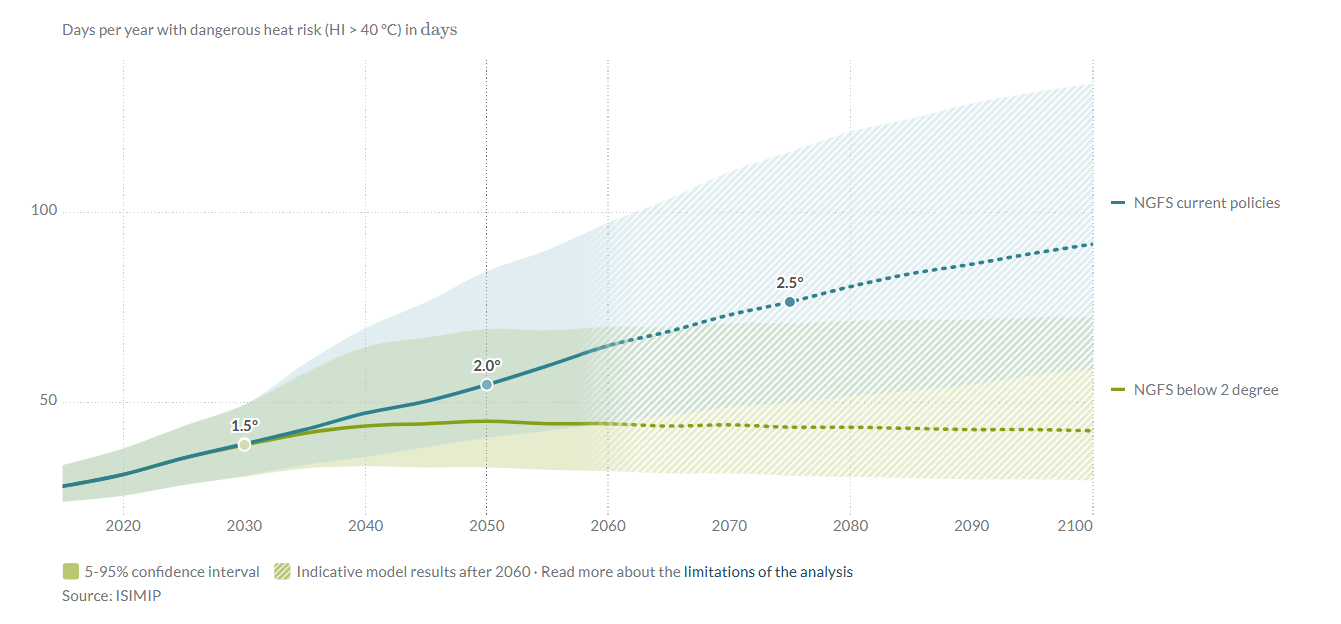
\includegraphics[width=0.9\linewidth,height=7.8cm,keepaspectratio]{cie_figure.png}
\caption*{\textbf{Figure 1. Days of dangerous heat per year in Niger.} The two pathways separate after 2030.
In 2100, the low end of the current-policies range (59 days) is above the central below-2\degC{} value
(42 days). Source: \CIE, Climate Analytics.}
\end{figure}
\vspace{-10pt}

\section{C. Assessment}
\begin{enumerate}[label=\arabic*.,start=7]
  \item Limiting warming below 2\degC{} avoids about 49 days of dangerous heat a year by 2100. It also cuts the
        rise in extreme rainfall from 43\,\% to 17\,\%. A 1.5\degC{} pathway keeps heat near today's level.
  \item Climate change could reduce Niger's annual GDP by 2.2\,\% to 11.9\,\% by 2050 (\WBtwentytwo).
  \item Drought increases in all scenarios. Adaptation is therefore needed now, whatever the outcome of the
        negotiations.
\end{enumerate}

\section{D. Recommendations}
\begin{enumerate}[label=(\alph*)]
  \item Support the 1.5\degC{} goal and national plans consistent with a rapid phase-out of fossil fuels.
  \item Link Niger's support for any agreement to more adaptation finance, with simple access for Least
        Developed Countries.
  \item Seek support from the Loss and Damage Fund for droughts and floods, with the African Group and the
        LDC Group.
  \item At home, fund drought-tolerant millet and sorghum, water harvesting and early warning systems.
\end{enumerate}

\section{E. Limits of the analysis}
\begin{enumerate}[label=\arabic*.,start=10]
  \item These figures are projections, not forecasts. Model ranges are wide, the drought indicator saturates,
        and the tool does not model millet or sorghum. Given Niger's vulnerability, real impacts are likely to
        be larger.
\end{enumerate}

% =====================================================================
%  REFERENCES (outside the 2-page limit)
% =====================================================================
\clearpage
\section{References}
{\singlespacing
\begin{list}{}{\leftmargin=1.4em \itemindent=-1.4em \itemsep=5pt \parsep=0pt}
\item AFP (2024, 9 October). Niger ups flood toll to 339 dead, more than 1 million affected.
      \emph{Inquirer.net}.
      \url{https://globalnation.inquirer.net/251812/niger-ups-flood-toll-to-339-dead-more-than-1-million-affected}
\item Climate Analytics (2026). \emph{Climate Impact Explorer}: Niger. Indicators: days per year with
      dangerous heat risk (HI > 40\degC), area under severe drought (SPEI < −1.5) and annual maximum 5-day
      precipitation; NGFS Below 2\degC, Current Policies and Net Zero 2050 scenarios; ISIMIP data.
      \url{https://climate-impact-explorer.climateanalytics.org} (accessed 9 October 2026).
\item Mohamed, A. M. L., Salack, S., Mkuhlani, S., Chemura, A., et al. (2025). Impact of climate change on
      millet yield under different fertilization levels in three agroecological zones of Niger Republic.
      \emph{PLOS ONE}, 20(10), e0333963. \url{https://doi.org/10.1371/journal.pone.0333963}
\item Sylla, M. B., Faye, A., Giorgi, F., Diedhiou, A., \& Kunstmann, H. (2018). Projected heat stress under
      1.5\degC{} and 2\degC{} global warming scenarios creates unprecedented discomfort for humans in West
      Africa. \emph{Earth's Future}, 6(7), 1029--1044. \url{https://doi.org/10.1029/2018EF000873}
\item Taylor, C. M., Belu\v{s}i\'{c}, D., Guichard, F., Parker, D. J., Vischel, T., Bock, O., Harris, P. P.,
      Janicot, S., Klein, C., \& Panthou, G. (2017). Frequency of extreme Sahelian storms tripled since 1982 in
      satellite observations. \emph{Nature}, 544, 475--478. \url{https://doi.org/10.1038/nature22069}
\item World Bank (2022). \emph{G5 Sahel Region Country Climate and Development Report}. CCDR Series.
      Washington, DC: World Bank. \url{http://hdl.handle.net/10986/37620}
\item World Bank (2024, 28 June). The World Bank supports food security and climate resilience for households
      in Niger [Press release].
      \url{https://www.worldbank.org/en/news/press-release/2024/07/01/the-world-bank-supports-food-security-and-climate-resilience-for-households-in-niger}
\end{list}}

\end{document}
